\documentclass{standalone}
\usepackage{tikz}
\usepackage{xcolor}
\usetikzlibrary{patterns, positioning}
\usetikzlibrary{shapes.misc}
\usepackage[outline]{contour}
\contourlength{1.5pt} 


\begin{document}
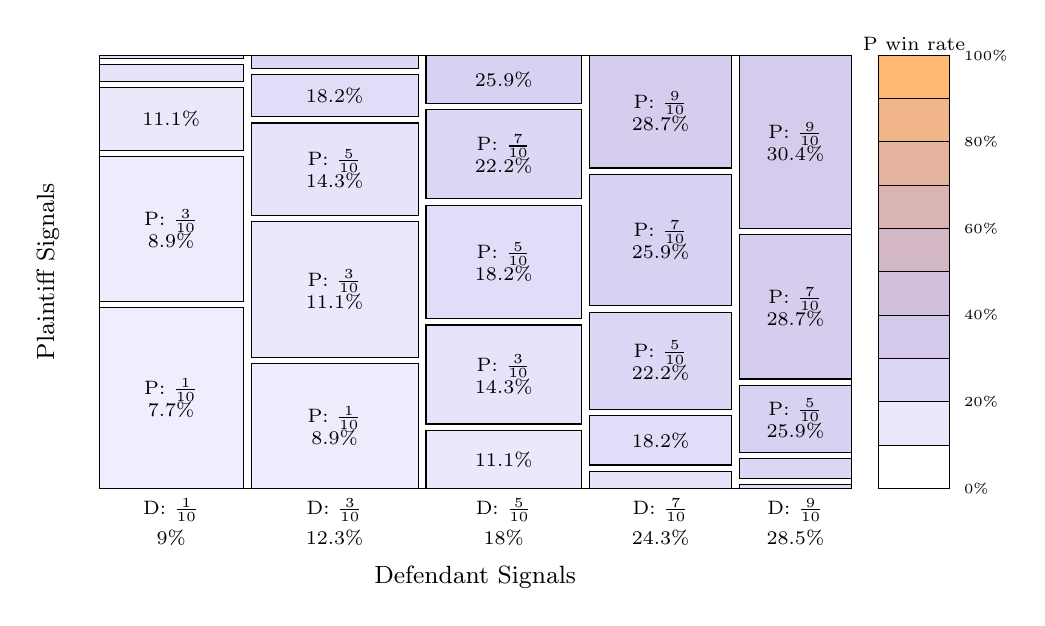
\begin{tikzpicture}
\newcommand{\DFractionOffset}{0.4}
\newcommand{\AxisLabelYAdjust}{-0.235}
\draw[draw=black] (0.6,2) rectangle (10.15,7.5);
\draw[fill=blue!92!orange!8!white!85!white, draw=black] (0.6,2) rectangle (2.4294,4.2945);
\draw (1.5147057646587492, 3.147229433591023) node[font=\scriptsize, text=black, align=center] {P: $\frac{1}{10}$\\ 7.7\%};
\draw[fill=blue!91!orange!9!white!85!white, draw=black] (0.6,4.3745) rectangle (2.4294,6.2106);
\draw (1.5147057646587492, 5.29250779163573) node[font=\scriptsize, text=black, align=center] {P: $\frac{3}{10}$\\ 8.9\%};
\draw[fill=blue!89!orange!11!white!84!white, draw=black] (0.6,6.2906) rectangle (2.4294,7.0872);
\draw (1.5147057646587492, 6.688881729832915) node[font=\scriptsize, text=black, align=center] {11.1\%};
\draw[fill=blue!86!orange!14!white!83!white, draw=black] (0.6,7.1672) rectangle (2.4294,7.3814);
\draw[fill=blue!82!orange!18!white!82!white, draw=black] (0.6,7.4614) rectangle (2.4294,7.5);
\draw (1.5147057646587492, 1.6) node[anchor=north, font=\scriptsize, text=black] {9\%};
\draw (1.5147057646587492, {1.6 + \DFractionOffset}) node[anchor=north, font=\scriptsize, text=black] {D: $\frac{1}{10}$};
\draw[fill=blue!91!orange!9!white!85!white, draw=black] (2.5294,2) rectangle (4.6511,3.5832);
\draw (3.590233079523995, 2.791598401515398) node[font=\scriptsize, text=black, align=center] {P: $\frac{1}{10}$\\ 8.9\%};
\draw[fill=blue!89!orange!11!white!84!white, draw=black] (2.5294,3.6632) rectangle (4.6511,5.3903);
\draw (3.590233079523995, 4.526763763697378) node[font=\scriptsize, text=black, align=center] {P: $\frac{3}{10}$\\ 11.1\%};
\draw[fill=blue!86!orange!14!white!83!white, draw=black] (2.5294,5.4703) rectangle (4.6511,6.6402);
\draw (3.590233079523995, 6.0552589171767535) node[font=\scriptsize, text=black, align=center] {P: $\frac{5}{10}$\\ 14.3\%};
\draw[fill=blue!82!orange!18!white!82!white, draw=black] (2.5294,6.7202) rectangle (4.6511,7.2533);
\draw (3.590233079523995, 6.986722768010234) node[font=\scriptsize, text=black, align=center] {18.2\%};
\draw[fill=blue!78!orange!22!white!81!white, draw=black] (2.5294,7.3333) rectangle (4.6511,7.5);
\draw (3.590233079523995, 1.6) node[anchor=north, font=\scriptsize, text=black] {12.3\%};
\draw (3.590233079523995, {1.6 + \DFractionOffset}) node[anchor=north, font=\scriptsize, text=black] {D: $\frac{3}{10}$};
\draw[fill=blue!89!orange!11!white!84!white, draw=black] (4.7511,2) rectangle (6.7253,2.7382);
\draw (5.738157736977849, 2.369110565658116) node[font=\scriptsize, text=black, align=center] {11.1\%};
\draw[fill=blue!86!orange!14!white!83!white, draw=black] (4.7511,2.8182) rectangle (6.7253,4.0754);
\draw (5.738157736977849, 3.446832699554016) node[font=\scriptsize, text=black, align=center] {P: $\frac{3}{10}$\\ 14.3\%};
\draw[fill=blue!82!orange!18!white!82!white, draw=black] (4.7511,4.1554) rectangle (6.7253,5.5962);
\draw (5.738157736977849, 4.87582401511301) node[font=\scriptsize, text=black, align=center] {P: $\frac{5}{10}$\\ 18.2\%};
\draw[fill=blue!78!orange!22!white!81!white, draw=black] (4.7511,5.6762) rectangle (6.7253,6.8113);
\draw (5.738157736977849, 6.2437677703739585) node[font=\scriptsize, text=black, align=center] {P: $\frac{7}{10}$\\ 22.2\%};
\draw[fill=blue!74!orange!26!white!79!white, draw=black] (4.7511,6.8913) rectangle (6.7253,7.5);
\draw (5.738157736977849, 7.1956658891568495) node[font=\scriptsize, text=black, align=center] {25.9\%};
\draw (5.738157736977849, 1.6) node[anchor=north, font=\scriptsize, text=black] {18\%};
\draw (5.738157736977849, {1.6 + \DFractionOffset}) node[anchor=north, font=\scriptsize, text=black] {D: $\frac{5}{10}$};
\draw[fill=blue!86!orange!14!white!83!white, draw=black] (6.8253,2) rectangle (8.6354,2.2165);
\draw[fill=blue!82!orange!18!white!82!white, draw=black] (6.8253,2.2965) rectangle (8.6354,2.9213);
\draw (7.730309025322184, 2.60886241211473) node[font=\scriptsize, text=black, align=center] {18.2\%};
\draw[fill=blue!78!orange!22!white!81!white, draw=black] (6.8253,3.0013) rectangle (8.6354,4.2393);
\draw (7.730309025322184, 3.6202945538866027) node[font=\scriptsize, text=black, align=center] {P: $\frac{5}{10}$\\ 22.2\%};
\draw[fill=blue!74!orange!26!white!79!white, draw=black] (6.8253,4.3193) rectangle (8.6354,5.9885);
\draw (7.730309025322184, 5.153892296321256) node[font=\scriptsize, text=black, align=center] {P: $\frac{7}{10}$\\ 25.9\%};
\draw[fill=blue!71!orange!29!white!79!white, draw=black] (6.8253,6.0685) rectangle (8.6354,7.5);
\draw (7.730309025322184, 6.784234317351006) node[font=\scriptsize, text=black, align=center] {P: $\frac{9}{10}$\\ 28.7\%};
\draw (7.730309025322184, 1.6) node[anchor=north, font=\scriptsize, text=black] {24.3\%};
\draw (7.730309025322184, {1.6 + \DFractionOffset}) node[anchor=north, font=\scriptsize, text=black] {D: $\frac{7}{10}$};
\draw[fill=blue!82!orange!18!white!82!white, draw=black] (8.7354,2) rectangle (10.15,2.05);
\draw[fill=blue!78!orange!22!white!81!white, draw=black] (8.7354,2.13) rectangle (10.15,2.38);
\draw[fill=blue!74!orange!26!white!79!white, draw=black] (8.7354,2.46) rectangle (10.15,3.3095);
\draw (9.442678603209579, 2.8847404906338556) node[font=\scriptsize, text=black, align=center] {P: $\frac{5}{10}$\\ 25.9\%};
\draw[fill=blue!71!orange!29!white!79!white, draw=black] (8.7354,3.3895) rectangle (10.15,5.2212);
\draw (9.442678603209579, 4.305307282378604) node[font=\scriptsize, text=black, align=center] {P: $\frac{7}{10}$\\ 28.7\%};
\draw[fill=blue!70!orange!30!white!78!white, draw=black] (8.7354,5.3012) rectangle (10.15,7.5);
\draw (9.442678603209579, 6.400580145401259) node[font=\scriptsize, text=black, align=center] {P: $\frac{9}{10}$\\ 30.4\%};
\draw (9.442678603209579, 1.6) node[anchor=north, font=\scriptsize, text=black] {28.5\%};
\draw (9.442678603209579, {1.6 + \DFractionOffset}) node[anchor=north, font=\scriptsize, text=black] {D: $\frac{9}{10}$};
\node[font=\small, text=black] at (5.375, {1.1 + \AxisLabelYAdjust}) {Defendant Signals};
\node[font=\small, text=black, rotate=90] at (-0.050000000000000044, 4.75) {Plaintiff Signals};
\draw[draw=black] (10.5,2) rectangle (11.4,7.5);
\draw (10.95, 7.65) node[font=\scriptsize, text=black] {P win rate};
\draw[fill=blue!100!orange!0!white!88!white, draw=black] (10.5,2) rectangle (11.4,2.55);
\draw[fill=blue!89!orange!11!white!84!white, draw=black] (10.5,2.55) rectangle (11.4,3.1);
\draw[fill=blue!78!orange!22!white!81!white, draw=black] (10.5,3.1) rectangle (11.4,3.65);
\draw[fill=blue!67!orange!33!white!77!white, draw=black] (10.5,3.65) rectangle (11.4,4.2);
\draw[fill=blue!56!orange!44!white!73!white, draw=black] (10.5,4.2) rectangle (11.4,4.75);
\draw[fill=blue!44!orange!56!white!70!white, draw=black] (10.5,4.75) rectangle (11.4,5.3);
\draw[fill=blue!33!orange!67!white!66!white, draw=black] (10.5,5.3) rectangle (11.4,5.85);
\draw[fill=blue!22!orange!78!white!62!white, draw=black] (10.5,5.85) rectangle (11.4,6.4);
\draw[fill=blue!11!orange!89!white!59!white, draw=black] (10.5,6.4) rectangle (11.4,6.95);
\draw[fill=blue!0!orange!100!white!55!white, draw=black] (10.5,6.95) rectangle (11.4,7.5);
\draw (11.46, 2) node[anchor=west, font=\tiny, text=black] {0\%};
\draw (11.46, 3.1) node[anchor=west, font=\tiny, text=black] {20\%};
\draw (11.46, 4.2) node[anchor=west, font=\tiny, text=black] {40\%};
\draw (11.46, 5.3) node[anchor=west, font=\tiny, text=black] {60\%};
\draw (11.46, 6.4) node[anchor=west, font=\tiny, text=black] {80\%};
\draw (11.46, 7.5) node[anchor=west, font=\tiny, text=black] {100\%};


\end{tikzpicture}
\end{document}